One of the main problems in the fake rate method used for the
\wjets\ background estimation is how to find an optimal threshold
requirement for the away jet in the QCD samples used to derive the
fake rate. Here we describe a method based on the idea of matching
energy in the isolation cone for \wjets\ same-sign events and the QCD
samples. 

For muon fakes we rely mostly on extrapolation in the isolation when
we define our loose (fakeable object) definition. Looking at the
isolation distribution we can see what QCD control sample has
isolation conditions similar to that of the \wjets\ fakes. The
variable used to measure the isolation energy deposition should be
either corrected for the pileup or be insensitive to it. We used the
2011 analysis definition of the isolation sum that has a minimum of 1
\GeV\ \pt\ requirement on the ECAL energy deposition, which
effectively makes it pileup independent. 

Figure~\ref{fig:appendix_fakeIso_ziso} shows the isolation energy
distribution for leptons from Z-decays, i.e. isolated muons. The
events are selected by requiring the ``fake'' muon to have
$\pt\in[10,15]\GeV$ and pass the muon fakeable object selection
requirements. For the other muon we used the tag selection
requirements used in the Tag-n-Probe studies. The dilepton mass is
required to be within 10~\GeV\ of the Z-boson
mass. Table~\ref{tab:appendix_fakeIso_stability} shows how the
distribution changed from one run period to the other. As one can see
the distribution is very stabled and the variable can be used for the
study.

Same-sign \wjets\ events can be selected quite easily in data. Beside
the charge requirement we just restrict ``fake'' $\pt<15\GeV$ and
$\met>30\GeV$ in the event. Figure~\ref{fig:appendix_fakeIso_fakeiso}
shows a comparison of the isolation energy deposition for the \wjets\
fakes and the ones from the different QCD samples in data. We find
that 30~\GeV\ away jet threshold is gives better agreement with
the \wjets\ distribution than 15~\GeV\ one.

\begin{table}
\begin{center}
\begin{tabular}{|l|c|c|}
\hline
Run period & Mean & RMS \\
\hline
Run 2012A & $0.064\pm0.002$ & $0.114\pm0.001$ \\
Run 2012B & $0.065\pm0.001$ & $0.118\pm0.001$ \\
Run 2012C & $0.065\pm0.001$ & $0.117\pm0.001$ \\
Run 2012D & $0.066\pm0.001$ & $0.119\pm0.001$ \\
\hline
\end{tabular}
\caption{Stability of the energy deposition in the isolation cone for \zmm\ events.} 
\label{tab:appendix_fakeIso_stability}
\end{center}
\end{table} 


\begin{figure}[!hbtp]
{
\centering
\subfigure[0-Jet]{
\centering
\label{fig:appendix_fakeIso_ziso}
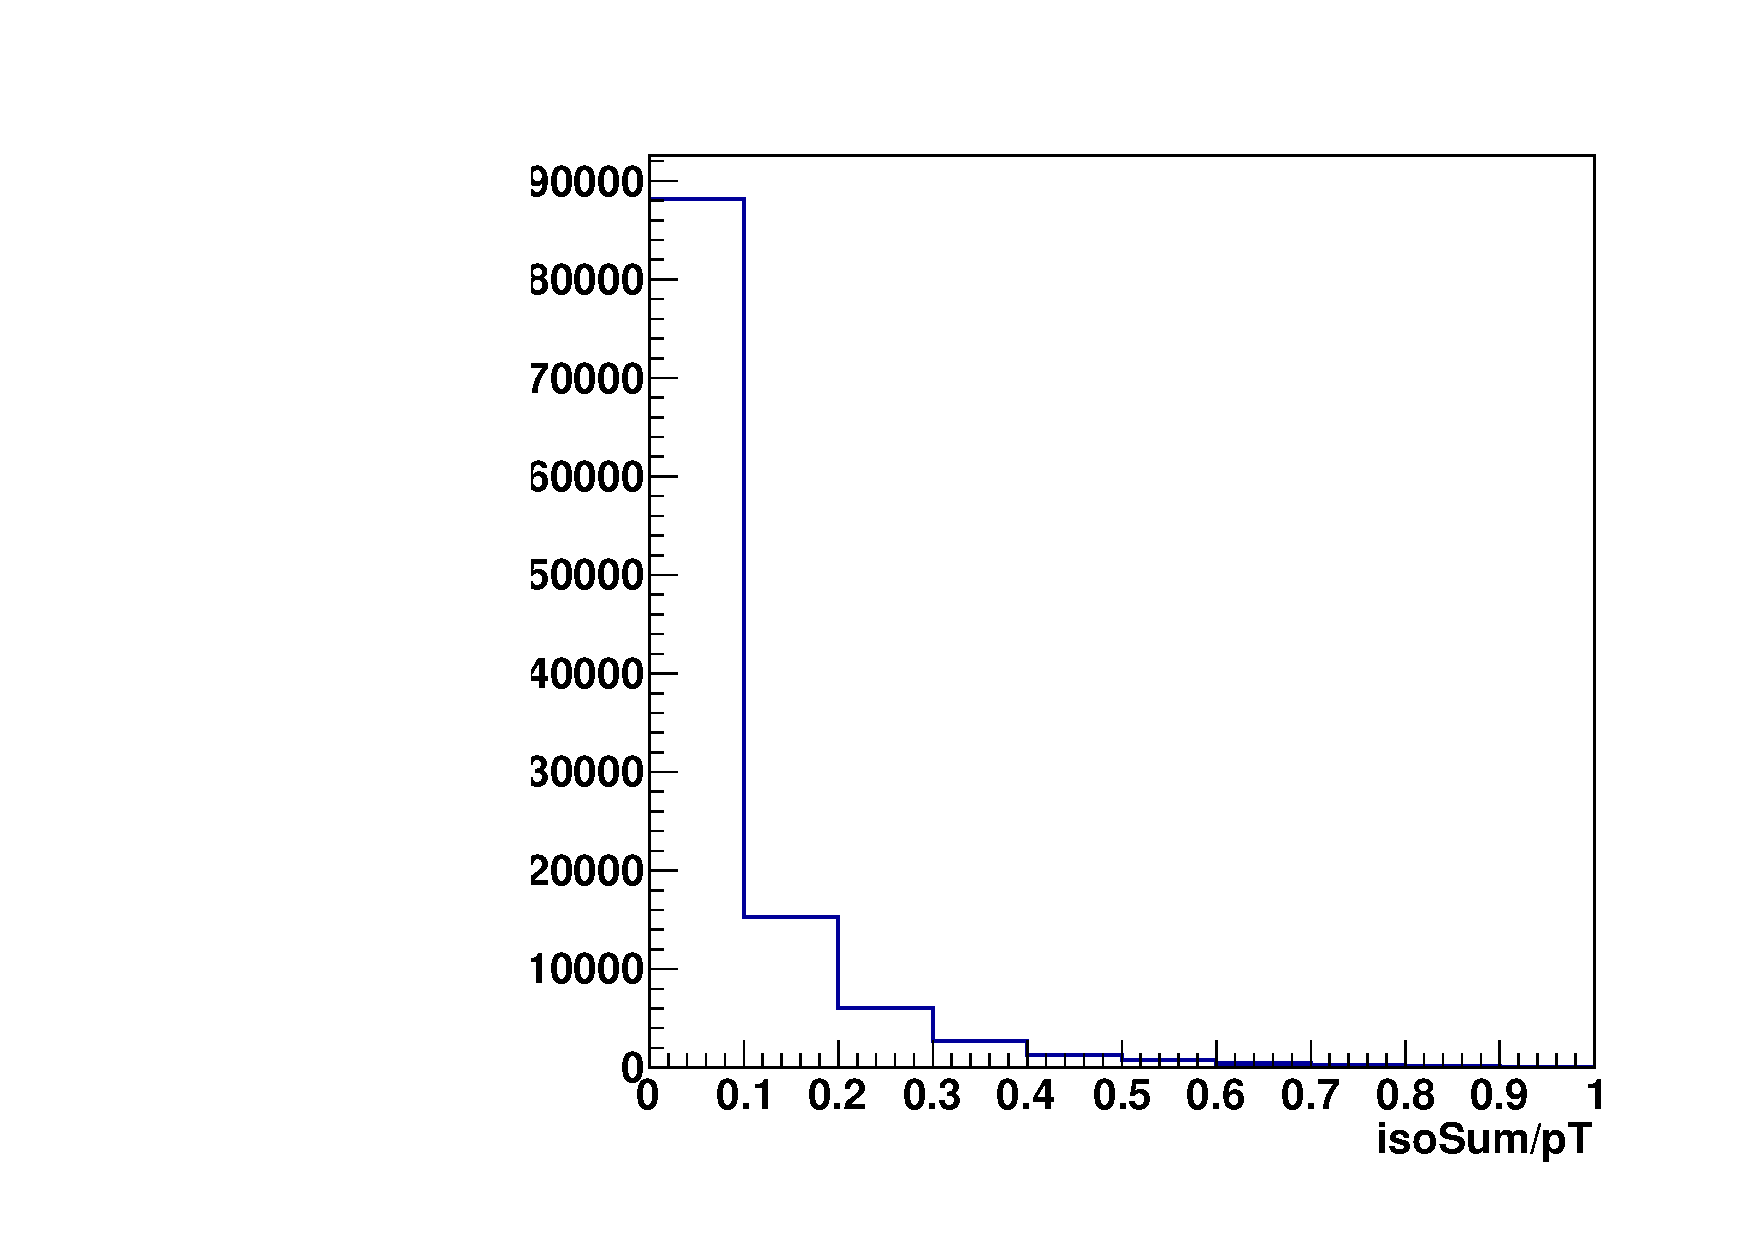
\includegraphics[width=.4\textwidth]{figures/appendix_fakeIso_z.pdf}
}
\subfigure[1-Jet]{
\centering
\label{fig:appendix_fakeIso_fakeiso}
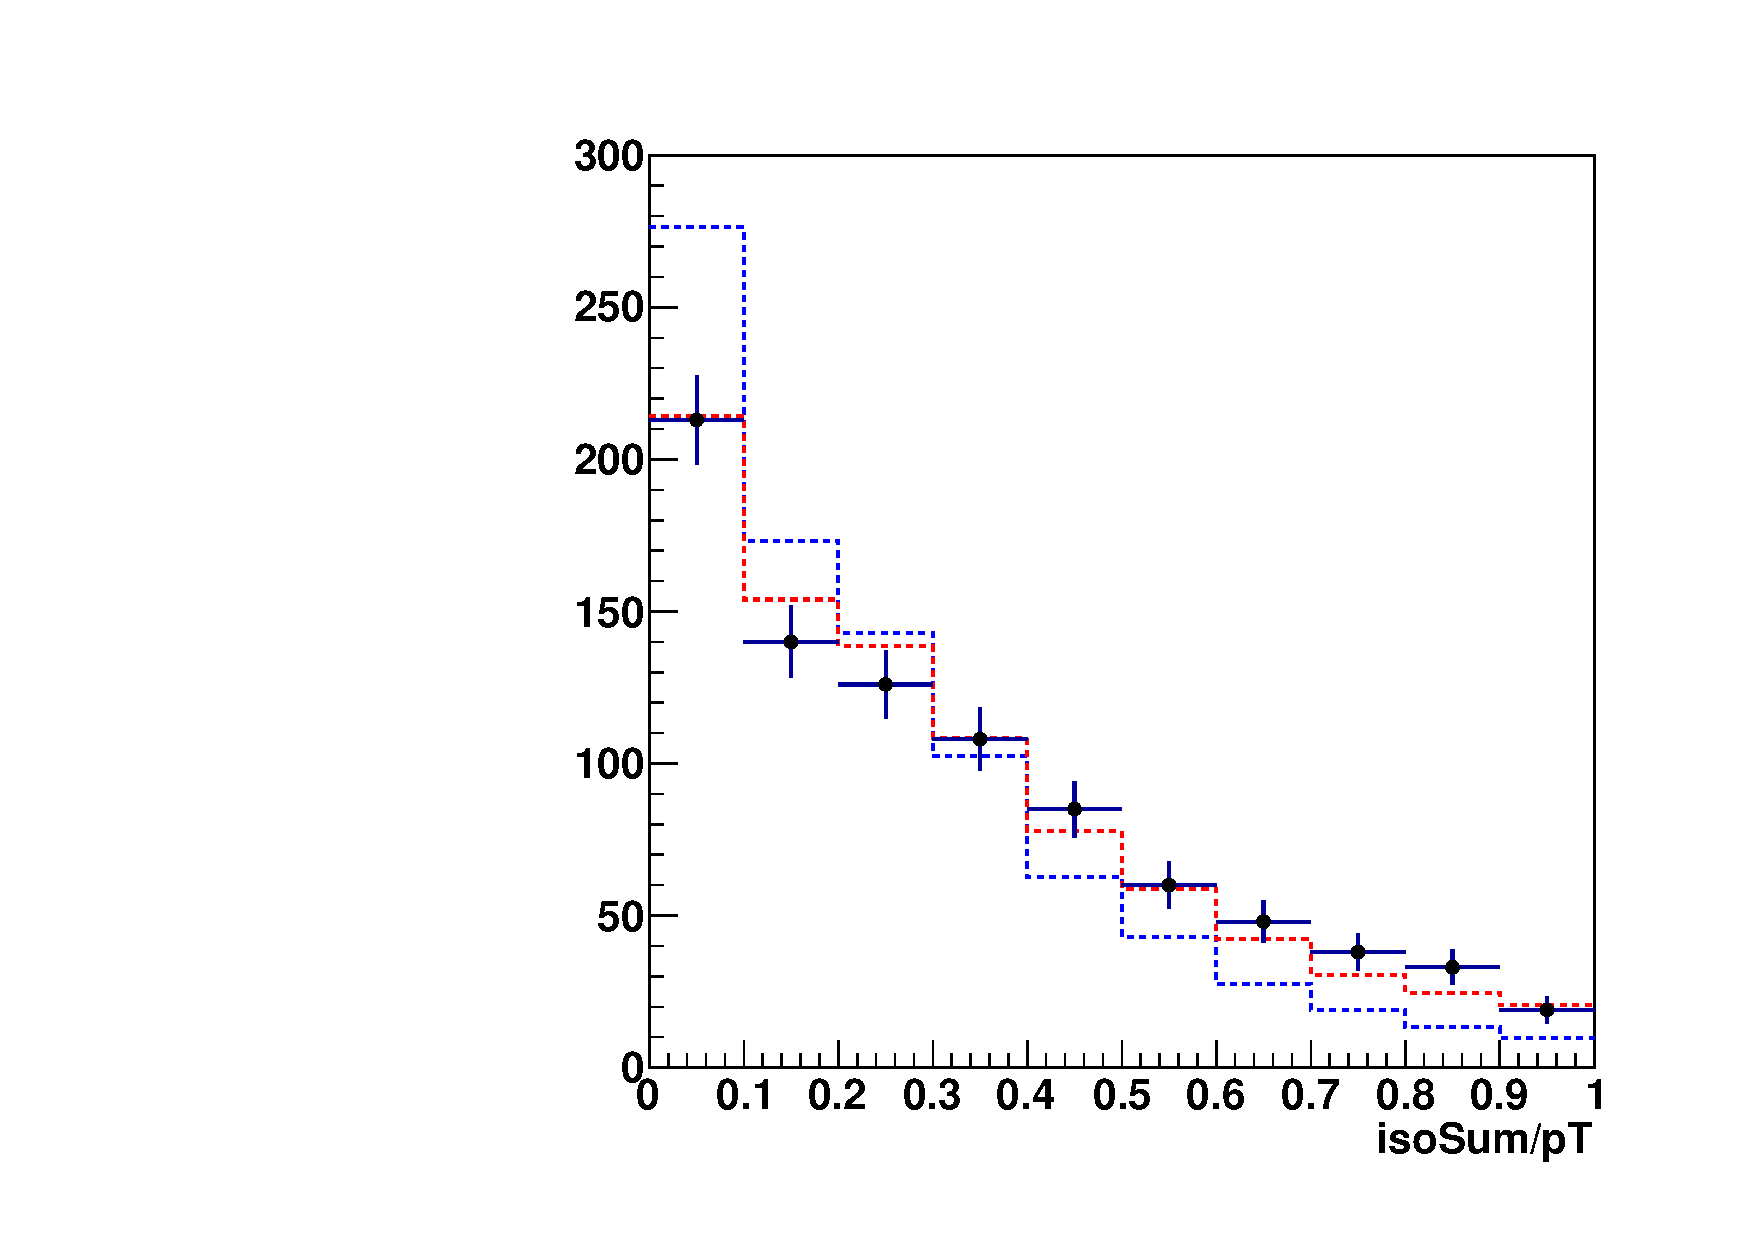
\includegraphics[width=.4\textwidth]{figures/appendix_fakeIso_fakes.pdf}
}\\
}
\caption{Left figure shows energy distribution in the isolation cone for \zmm\ events. 
Right figure shows the energy distribution for \wjets\ same-sign fakes (dots), overlaid 
with QCD 15 (blue dashed line} and QCD 30 (red dashed line) histograms.

\end{figure}


